\documentclass[times, utf8, seminar, numeric]{fer}

\usepackage{booktabs}
\usepackage{hyperref}
\usepackage{graphicx}
\usepackage{fancyhdr}
\usepackage{float}
\hypersetup{
	colorlinks=true,
	linkcolor=black,
	filecolor=magenta,      
	urlcolor=cyan,
	pdftitle={Overleaf Example},
	pdfpagemode=FullScreen,
}
\begin{document}


\title{Praćenje nogometaša primjenom YOLOv5 modela i DeepSORT algoritma}

\author{Marko Tutić}
\voditelj{Izv. prof. dr. sc. Zoran Kalafatić}
\maketitle

\tableofcontents

\chapter{Uvod}



Praćenje objekata je grana računalnog vida u kojoj se detekcije zadane u određenom okviru nastoje pratiti u nadolazećim okvirima.
Metode praćenja objekata se najčešće razvrstavaju u metode praćenja jednog objekta i metode praćenja više objekata. 
U metode praćenja jednog objekta ubrajaju se metode koje ne zahtjevaju zadavanje detekcija u svakom okviru videozapisa. U takvim metodama dovoljno je zadati poziciju objekta u nekom početnom okviru, a metoda zatim može pratiti objekt u daljnjim okvirima isključivo na temelju karakteristika objekata i promjena koje se događaju u slici.

Praćenje više objekata se realizira kao detektiranje objekata i dodijeljivanje identifikatora detekcijama na temelju prethodnih detekcija te je cilj očuvati ispravne identifikacije objekata kroz više okvira videozapisa. Ove metode zahtjevaju detekcije u svakom okviru videozapisa.
Praćenje više objekata često se vodi pretpostavkom da objekti neće naglo mijenjati brzinu i smjer kretanja.

Praćenje više objekata predstavlja veliki izazov u području računalnog vida jer se redovito javljaju situacije koje mogu izazvati propuštanje dodijeljivanja identifikatora ili pogrešno dodijeljivanje identifikatora poput zaklanjanja objekta i zamjene identiteta.
Zaklanjanje objekta je pojava kada objekt nije vidljiv na slici, ali se pozicija objekta i dalje nalazi unutar slike.
Do zamjene identiteta dolazi kada se objekti mimoilaze ili se nalaze vrlo blizu određeno vrijeme te se kao posljedica toga identitet jednog objekta dodijeli drugom i obrnuto. 

Praćenje nogometaša predstavlja situaciju u kojoj je potrebno pratiti više objekata pri čemu su zamjene identiteta česte s obzirom da se igrači kroz trajanje cijele utakmice mimoilaze i zaklanjaju na kameri. Dodatan izazov pri praćenju nogometaša predstavlja činjenica da igrači izgledaju vrlo slično na velikoj udaljenosti zbog identičnih boja dresova.



Originalni SORT algoritam za praćenje objekata imao je problem sa velikim brojem zamjena identita s obzirom da je uzimao u obzir samo pozicije objekata prilikom dodijeljivanja identiteta. 
DeepSORT algoritam nastoji rješiti taj problem uvođenjem duboke metrike asocijacije koja se temelji na opisnicima izgleda objekata koji generiraju vektor karakteristika koji opisuje izgled za svaki objekt. Taj vektor se također razmatra prilikom izračuna udaljenosti detekcija i predviđenih trajektorija.

DeepSORT algoritam zahtjeva detekcije objekata u svakom okviru kako bi korigirao svoja interna stanja koja koristi za predviđanje novih trajektorija. Za detekciju nogometaša koristi se YOLOv5s model koji je naučen na specifičnom skupu podataka. 
Dobivene detekcije se prosljeđuju algoritmu za praćenje objekata.

Pozicije nogometaša u nekom okviru bilježe se za svakog nogometaša zasebno te se na temelju tih pozicija izrađuje mapa aktivnosti igrača. Pozicija nogometaša se tretiraju kao slučajna varijabla pri čemu je mapa aktivnosti vizualizacija funkcije gustoće te varijable. Za izradu mape aktivnosti koristi se procjena parametara gustoće jezgrom (kernel density estimate) koja koristi pozicije igrača za procjenu funkcije gustoće.



\chapter{Skup podataka}

Za skup podataka na kojem se vrši učenje i testiranje sustava iskorišten je videozapis duljine 5 minuta koji sadrži snimku jedne nogometne utakmice. Kamera kojom je utakmica snimana je statična. Svi okviri u videozapisu sadrže pregled cijelog nogometnog terena.
Jedna sekunda navedenog videozapisa sadrži 25 slikovnih okvira. 
Širina videozapisa iznosi 3260 piksela dok visina okvira videozapisa iznosi 570 piksela.
Slika \ref{fig:okvir} prikazuje primjer jednog okvira iz videozapisa

\begin{figure}
	\centering
	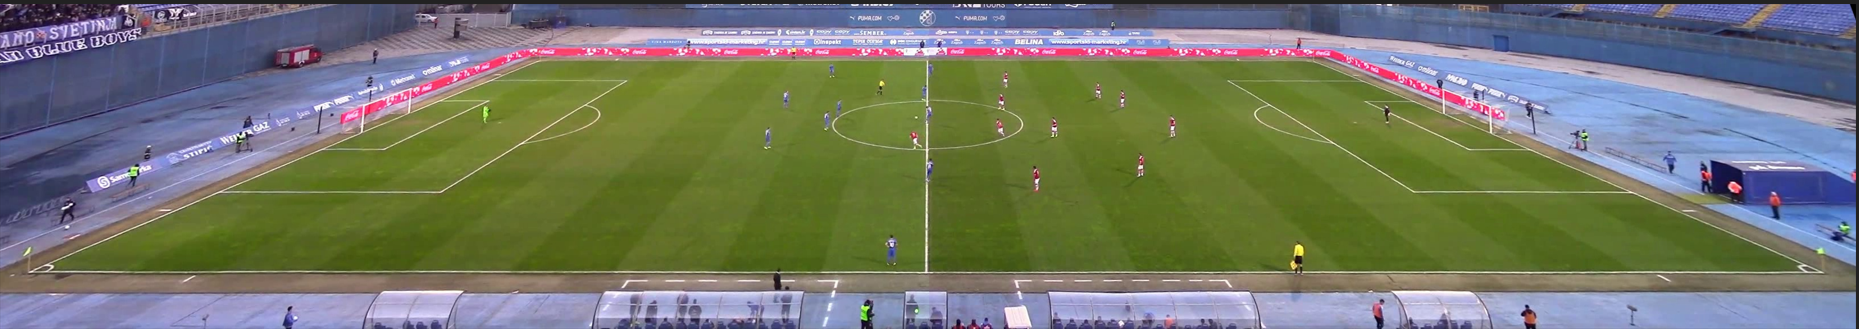
\includegraphics[width=\linewidth]{slike/okvir.png}
	\caption {Primjer okvira iz videozapisa}
	\label{fig:okvir}	
\end{figure}


Skup podataka dodatno sadrži tekstualni dokument koji sadrži pozicije i identifikatatore igrača i sudca. Oznake su zapisane u obliku propisanom MOT16 specifikacijom. Jedan redak teksutalne datoteke ima sljedeći format:

\textit{<redni broj okvira>, <identifikator igraca>, <x koordinata>, <y koordinata>, <širina>, <visina>, -1, -1, -1, -1.}

Slika \ref{fig:oznake} prikazuje primjer oznaka pozicija i identifikatora igrača za prvi okvir videozapisa.

\begin{figure}
	\centering
	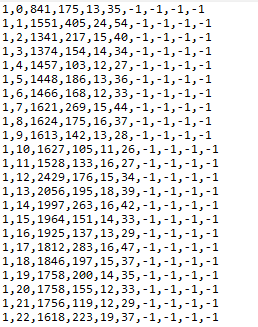
\includegraphics[scale=0.8]{slike/oznake.png}
	\caption {Primjer oznaka skupa podataka}
	\label{fig:oznake}	
\end{figure}



Koordinate x i y te širina i visina odnose se na pravokutnik koji omeđuje igrača na slici. Koordinate x i y označuju poziciju gornje lijeve točke takvog pravokutnika. Na temelju širine i visine mogu se izvesti i ostale točke omeđujućeg pravokutnika.
Niz brojeva -1 se ne koristi, no služe kao nadopuna za zadovoljavanje MOT specifikacije.

Skup podataka dijeli se na skup za učenje, skup za provjeru i skup za testiranje. 
Okviri videozapisa se dijele u navedene skupove slijedno kako bi se očuvala mogućnost praćenja objekata u navedenim skupovima podataka. 
Za potrebe učenja detektora objekata oznake koje su zadane u MOT16 formatu potrebno je pretvoriti u oznake koje zadovoljavaju YOLOv5 format oznaka. YOLOv5 format propisuje izradu tekstualne datoteke s oznakama za svaki okvir te se omeđujući pravokutnik opisuje središtem tog pravokutnika i njegovom širinom i visinom. Identifikatori igrača se ne uzimaju u obzir prilikom pretvorbe jer detektor objekata samo treba lokalizirati objekte te ih klasificirati. Pretvorba gornje lijeve točke u središnju točku pravokutnika vrši se primjenom sljedećih formula:
\[x^{'} = x + \frac{width}{2}\] 
\[y^{'} = y + \frac{height}{2}\] 

Skup podataka se dijeli tako da skup za učenje sadrži prvih 4500 okvira videozapisa, skup za validaciju sadrži idućih 1500 okvira, dok skup za testiranje sadrži preostalih 1515 okvira. 

Skup za učenje koristi se za učenje modela detekcije objekata. 
Skup za validaciju koristi se za provjeru svojstva generalizacije tijekom različitih epoha prilikom učenja modela detekcije objekata. 
Konačno, skup za testiranje koristi za evaluaciju modela detektora objekata nakon što je završen proces učenja. 

Iako se u DeepSORT algoritmu za praćenje objekata može naučiti opisnik izgleda objekata pomoću istog skupa podataka, taj postupak će biti preskočen s obzirom da izvorni algoritam već sadrži opisnik izgleda osoba koji je prethodno naučen na MARS (Motion Analysis and Re-Identification Set) skupu podataka koji sadrži slike različitih osoba. Takav opisnik izgleda naučen je za izlučivanje značajki koje opisuju izgled jedne osobe. 
Sustav za praćenje objekata će se samo testirati na skupovima za učenje i testiranje.


% TODO dodaj sliku videozapisa i formata tekstualne datoteke


\chapter{Arhitektura sustava}

Sustav za praćenje nogometaša i generiranje mape aktivnosti sastoji se od 3 komponente:
\begin{itemize}
	\item Podsustav za detekciju pozicija nogometaša u okviru
	\item Podsustav za praćenje nogometaša između okvira
	\item Podsustav za generiranje mape aktivnosti na temelju rezultata dobivenih praćenjem nogometaša
\end{itemize}


\section{Detekcija nogometaša}
Za detekciju nogometaša na slici koristi se YOLOv5s model iz skupa modela YOLOv5. Karakteristike YOLOv5 modela je da sliku podijeli na ćelije te je svaka ćelija zadužena za detektiranje objekata kojima se središte nalazi u toj ćeliji. Sustav na ulazu prima slike koje predstavljaju okvire videozapisa te na izlazu vraća skup detekcija objekata na slici. Model vraća uvijek isti broj detekcija te je potrebno ukloniti redundantne detekcije primjenom algoritma potiskivanja nemaksimalnih odziva (engl. non-maximum surpression). S ozbirom da se na terenu većinu vremena nalazi 22 nogometaša i jedan sudac, očekivani broj detekcija u svakom okviru iznosi 23. Model za detekciju objekata služi isključivo za određivanje pozicija nogometaša u trenutnom okviru, odnosno ne može identificirati pojedine objekte jer ne uzima u obzir detekcije iz prethodnih okvira. 	














\pagebreak
\section{Praćenje objekata}
Za praćenje objekata koristi se algoritam DeepSORT.

Algoritam DeepSORT nastao je kao proširenje SORT algoritma koji se bazirao na korištenju Kalmanovog filtra za predviđanje trajektorija te mađarskog algoritma za dodijelu detekcija trajektorijama na temelju njihovog omjera presjeka i unije. Iako je takav algoritam imao veliku brzinu izvođenja, zamjena identiteta je bila česta pojava. Algoritam DeepSORT nastoji rješiti taj problem uvođenjem opisnika izgleda objekta koji se također uzima u obzir prilikom dodjele detekcija trajektorijama. Arhitektura mreže za dobivanje opisnika izgleda objketa prikazana je tablicom na Slici \ref{fig:deep_sort_net_arch}.
  
Algoritam također koristi Kalmanov filtar u svakoj trajektoriji za praćenje trenutnog stanja i predviđanje idućeg stanja, odnosno pozicije trajektorije u sljedećem okviru videozapisa. 
Predviđene trajektorije se uspoređuju sa detekcijama sa izlaza detektora objekata te se na temelju međusobne udaljenosti uparuju.
Udaljenost se definira kao težinska suma Mahalanobisove udaljenosti trajektorije i detekcije te kosinusne udaljenosti opisnika izgleda detekcije i trajektorije. 

Uparivanje se vrši primjenom kaskadnog uparivanja koje se bazira na iterativnoj primjeni Mađarskog algoritma pri čemu se prilikom uparivanja daje prioritet češće ažuriranim trajektorijama. Rezultat algoritma su uparene detekcije i trajektorije. Arhitektura sustava prikazana je na Slici \ref{fig:deep_sort_arch}.




\begin{figure}
	\centering
	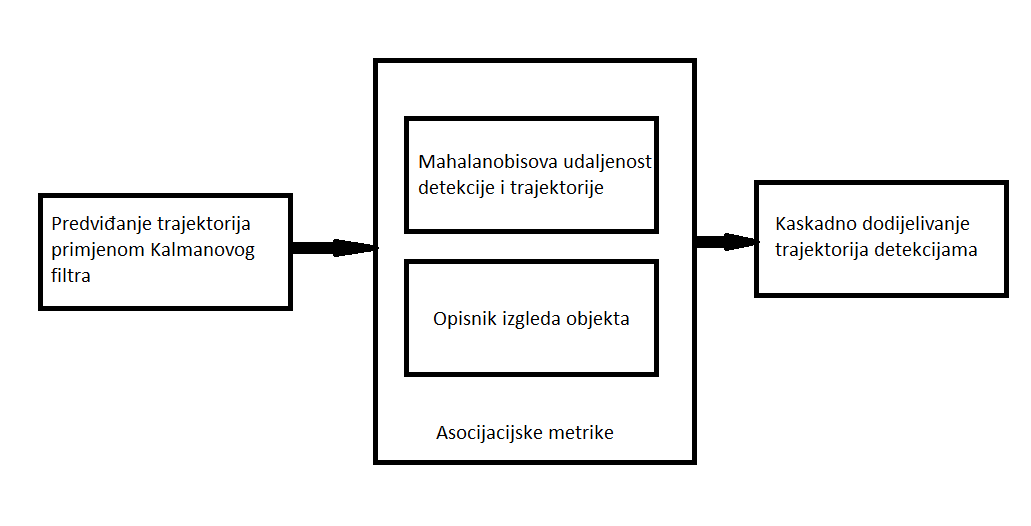
\includegraphics[scale=0.6]{slike/deep_sort_arch.png}
	\caption {Arhitektura DeepSORT algoritma}
	\label{fig:deep_sort_arch}	
\end{figure}

\begin{figure}
	\centering
	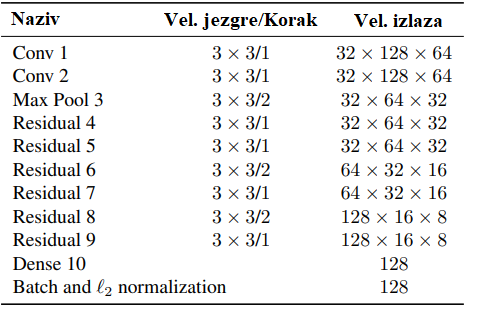
\includegraphics[scale=0.5]{slike/deep_sort_net_arch.png}
	\caption {Arhitektura opisnika izgleda}
	\label{fig:deep_sort_net_arch}
\end{figure}


\subsection{Kalmanov filtar}

Kalmanov filtar se u algoritmu DeepSORT koristi za praćenje internog stanja trajektorije te predviđanje pozicije objekta ukoliko detektor objekta ne uspije detektirati praćeni objekt u novom okviru. Interno stanje trajektorije se ažurira kada god je dostupan vektor mjerenja. Vektor mjerenja u kontekstu ovog algoritma jednak je jednoj detekciji objekta. 

Algoritma DeepSORT stanje trajektorije definira kao 8-dimenzionalni vektor koji se sastoji od: x koordinate objekta, y koordinate središta objekta, omjera visine i širine, visine te brzina promjena za svaku od prethodno navedenih komponenti. Mjerenje se definira kao 4-dimenzionalni vektor koji se sastoji od: x koordinate pozicije objekta, y koordinate pozicije objekta, omjera visine i širine omeđujućeg pravokutnika detekcije te visine tog pravokutnika. 


Za detekcije koje nisu uparene s postojećim trajektorijama prlikom procesa uparivanja, stvaraju se nove trajektorije koje su na početku u stanju pripravnosti, odnosno još se ne tretiraju kao rezultat praćenja objekata. Tek ukoliko se novostvorenoj trajektoriji dodijeli mjerenje kroz određen broj uzastopnih okvira, trajektorija prelazi u aktivno stanje te se tek tada tretira kao ispravna trajektorija. Na taj način se spriječava praćenje nepostojećih objekata \cite{deepsort}.

Kada je trajektorija u aktivnom stanju te vektor mjerenja nije dostupan, odnosno detekcija nije dodijeljena, sljedeće stanje se predviđa pomoću internog stanja trajketorije \cite{sort}.
Ukoliko se nekoj aktivnoj trajektoriji ne dodijeli mjerenje unutar određenog broja uzastopnih okvira, trajektorija i njeno stanje se briše. \cite{deepsort}.

% TODO opiši linearan model predviđanja stanja ako bude potrebno.

\subsection{Dodjela trajektorija detekcijama}

U svakom okviru potrebno je dodijeliti detekcije trajektorijama tako da parovi detekcija i trajektorija budu minimalno udaljeni.
Algoritam DeepSORT ne pokušava upariti sve detekcije i trajektorije odjednom već daje prednost trajektorijama kojima se interno stanje češće ažurira pomoću novih mjerenja, odnosno detekcija. 
Algoritam kreće od dodijelivanja nedodijeljenih detekcija najčešće ažuriranim trajektorijama. 

Kriterij koji se razmatra prilikom uparivanja trajektroija i detekcija sastoji se od dvije komponente: kvadrirane mahalanobisove udaljenost između predviđene pozicije objekta (dobiva se primjenom Kalmanovog filtra) i detekcije te minimalne kosinusne udaljenosti između opisnika izgleda detektiranog objekta i prethodnih opisnika objekta za određenu trajektoriju. Za jednu trajektoriju se pamti određen broj opisnika izgleda detekcija koje su bile prethodno uparene s tom trajektorijom. Prethodno navedene udaljenosti se linearno kombiniraju u konačnu udaljenost koja se razmatra prilikom dodijele detekcija trajektorijama.

Trajektorije i detekcije s minimalnom udaljenošću uparuju uzimajući u obzir ažurnost trajektorija i prag udaljenosti koji mora biti zadovoljen. Rezultat uparaivanja s ovim ograničenjima je da će neke trajektorije biti uparene s nekim detekcijama, ali i dalje mogu ostati neuparane detekcije i neuparene trajektorije. U idućem koraku se ponovo uzimaju nove neuparene trajektorije koje su rijeđe ažurirane od prethodno uparenih te se pokušavaju upariti s preostalim neuparenim detekcijama. 

Kao parametar algoritma se postavlja maksimalni broj okvira, odnosno maksimalno vrijeme koje je prošlo od ažuriranja trajektorije te se ono koristi za određivanje koliko puta će pokušati dodijeliti neuparene detekcije neuparenim trajektorijama. 

Ako nakon ovakvog iterativnog dodjeljivanja i dalje postoje neuparene detekcije i trajektorije, one se uparuju primjenom Mađarskog algorima gdje se kao kriterij optimizacije prilikom dodjeljivanja koristi omjer presjeka i unije između područja detekcije i predviđenog područja trajektorije. Za ovo dodjeljivanje se također uvodi prag koji mora biti zadovoljen kako bi se uparivanje smatralo uspješnim\cite{deepsort}.

Ukoliko i dalje postoje neuparane detekcije, za njih se stvaraju nove trajektorije koje zatim moraju proći fazu pripravnosti. Neuparene trajektorije ne dobivaju mjerenje u tom okviru te ukoliko su u aktivnom stanje, same predviđaju svoju poziciju primjenom kalmanovog filtra.

% TODO dodaj formule za udaljenosti

\section{Izrada mape aktivnosti}

Mape aktivnosti izrađuju se nakon analize cijelog videozapisa. Pozicije praćenih objekata zapisane su u tekstualnoj datoteci te se one zapisuju u skladu s MOT16 formatom. Mape aktivnosti se izrađuju za svakog nogometaša zasebno te se pohranjuju kao slike. 

Za izradu mape aktivnosti, koristi se slika igrališta iz ptičje perspektive kao pozadina. Navedena slika prikazana je na Slici \ref{fig:pitch}. 

\begin{figure}
	\centering
	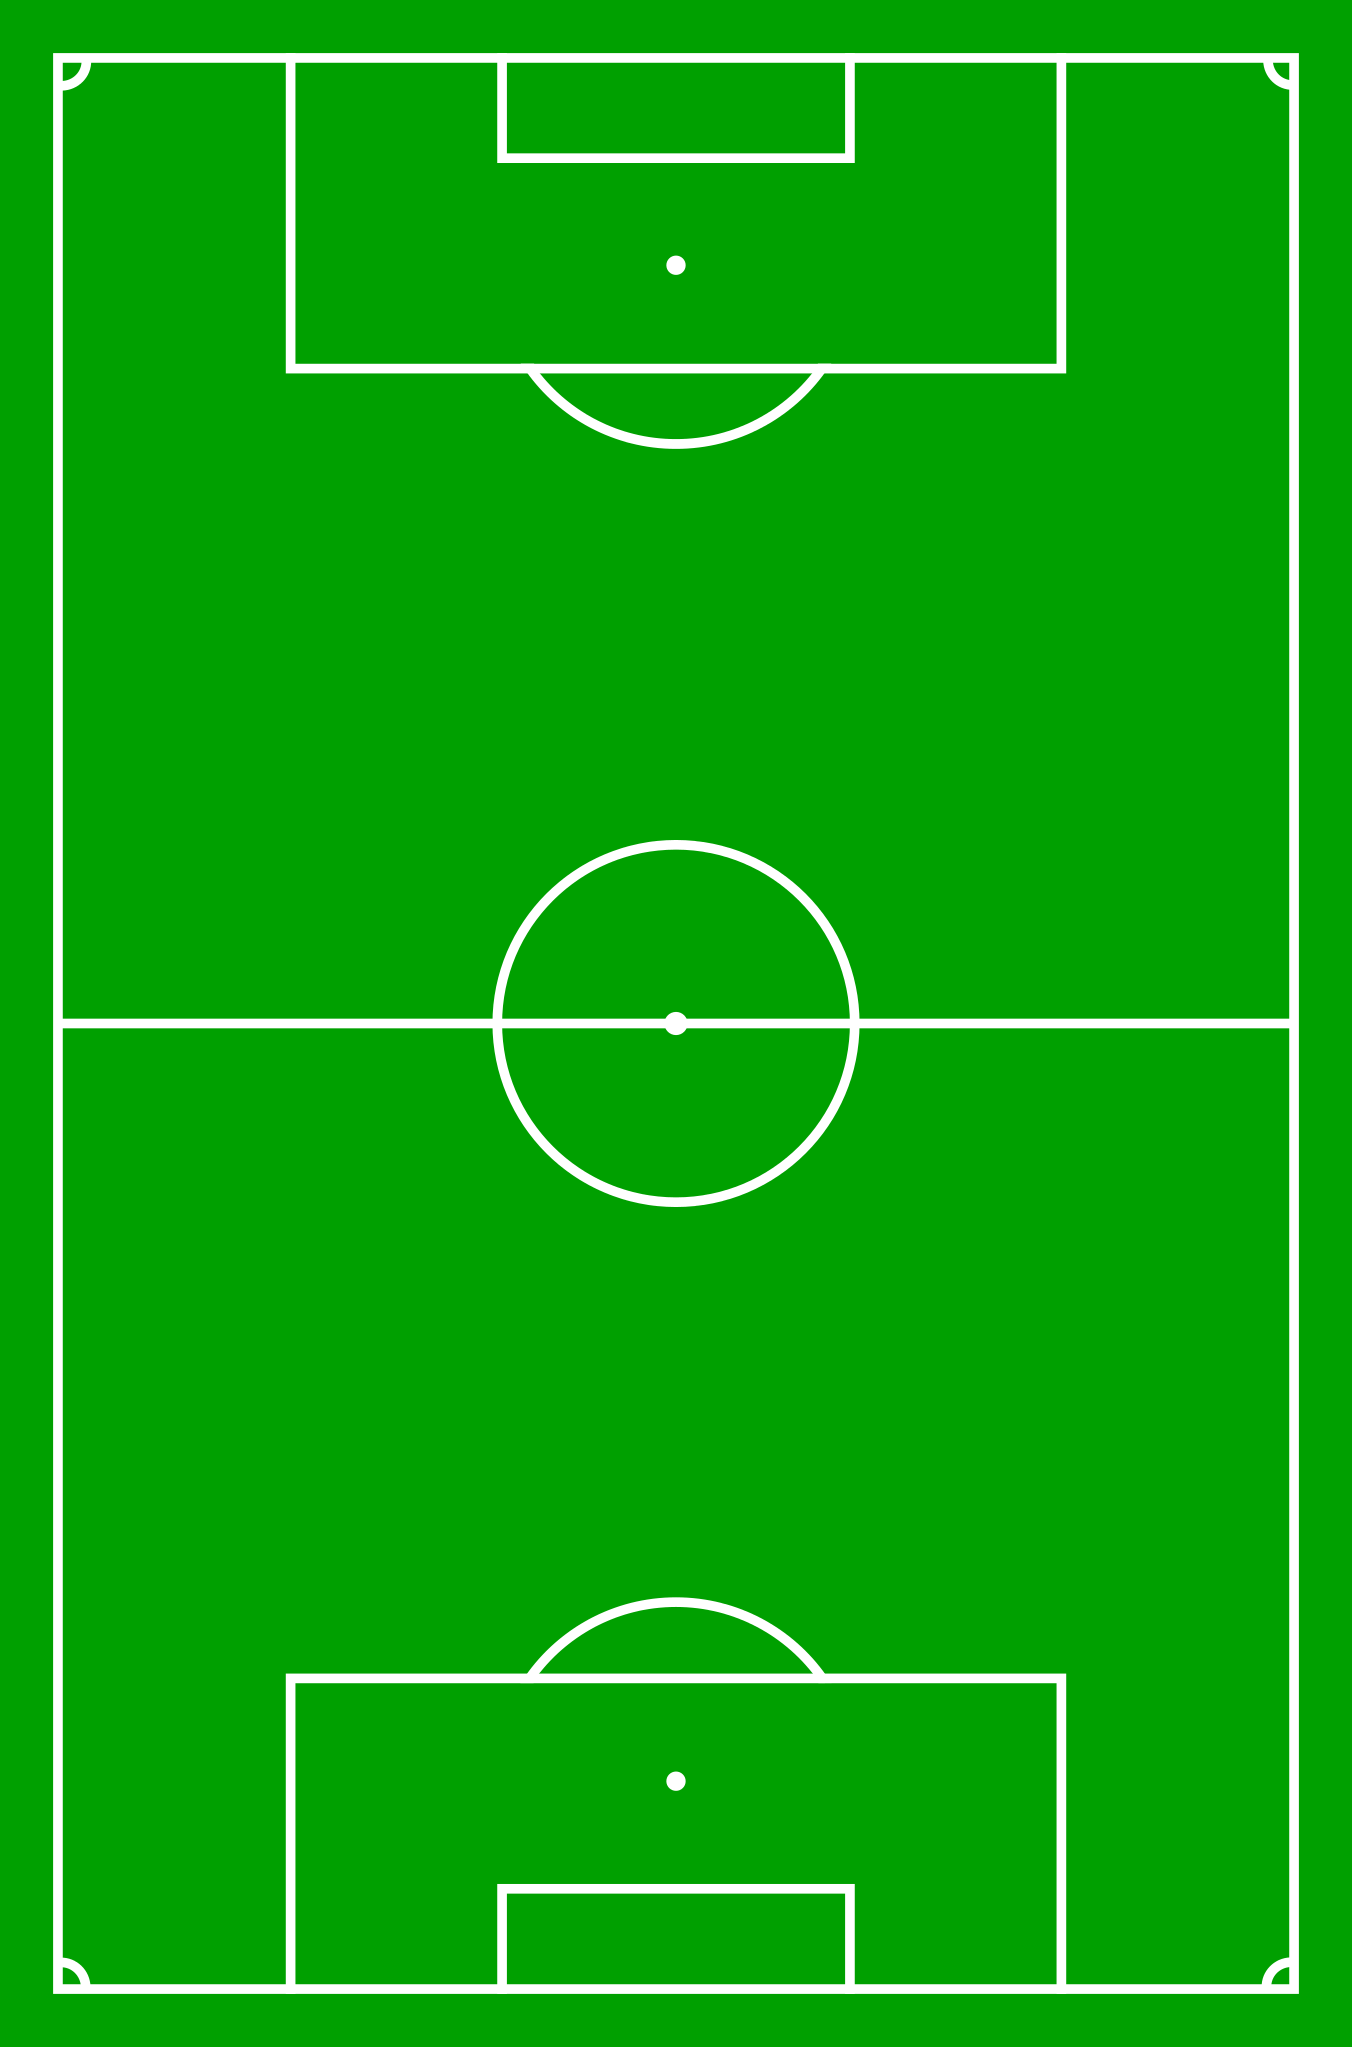
\includegraphics[scale=0.15]{slike/pitch.png}
	\caption {Nogometni teren iz ptičje perspektive}
	\label{fig:pitch}	
\end{figure}

Na početku se za svakog igrača izrađuju se liste x i y koordinata njihovih pozicija na okvirima videozapisa. Pozicije igrača na okvirima videozapisa ne moraju odgovarati pozicijama na slici terena iz ptičje perspektive te je stoga potrebno provesti perspektivnu transformaciju. Za poziciju igrača odabrana je točka koja se nalazi na polovištu donje lijeve i donje desne točke omeđujućeg pravokutnika detekcije igrača.
 
Za dobivanje matrice perspektivne transformacije potrebno je zadati četiri točke koje predstavljaju pozicije rubova igrališta u videozapisu te četiri točke koje predstavljaju rubove igrališta na slici terena iz ptičje perspektive. 

Na temelju tih točaka izračunava se transformacijska matrica pomoću koje se sve točke koje predstavljaju poziciju igrača na okviru videozapisa preslikavaju u poziciju igrača na terenu snimljenom iz ptičje perspektive. S obzirom da se pozicija kamere može razlikovati u videozapisima, potrebno je za svaki videozapis precizno zadati točke koje predstavljaju rubove terena, jer će u protivnom rezultirajuće mape aktivnosti biti netočne.

Jednom kada su sve točke pozicija u okvirima preslikane u odgovarajuće točke pozicija na terenu iz ptičje perspektive, izračunava se mapa aktivnosti. Pozicije nogometaša tretiraju se kao slučajne varijable koje imaju nepoznatu funkciju gustoće. Za procjenu te razdiobe koristi se procjena pomoću jezgre. Konačan rezultat je procjenjena funkcija gustoće pozicija koja ujedno predstavlja i mapu aktivnosti nekog igrača. Primjer jedne mape aktivnosti prikazan je na Slici \ref{fig:heatmap}

\begin{figure}
	\centering
	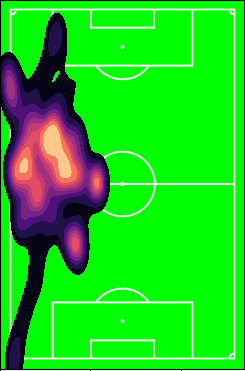
\includegraphics[scale=1]{slike/heatmap.png}
	\caption {Mapa aktivnosti za igrača}
	\label{fig:heatmap}	
\end{figure}


\chapter{Implementacija sustava}

\section{Podsustav za detekciju nogometaša}


Podsustav za detekciju nogometaša sastoji se YOLOv5 detektora objekata koji na ulazu prima slikovne okvire videozapisa, a na izlazu vraća detekcije sa prikladnim podacima o detekciji. 
Implementacija YOLOv5 detektora preuzeta je sa izvornog repozitorija \cite{yolov5impl}. U repozitoriju se nalaze skripte za učenje modela detekcije kao i za vrednovanje modela dobivenog učenjem. Dodatno se prilikom implementacije sustava praćenja nogometaša iz repozitorija iskorištavaju funkcije za potiskivanje nemaksimalnih odziva, označavanje izlaznih detekcija na slikama, dohvaćanje treniranog modela te provođenje detektiranja objekata u slikovnom okviru. 
Potiskivanje nemaksimalnih odziva (engl. non-maximum surpression) potrebno je provesti kako bi se uklonile redundantne detekcije, tj. detekcije niske pouzdanosti i višestruke detekcije. 



Detektor objekata YOLOv5 zahtjeva skup podataka za učenje, provjeru i testiranje u specifičnom formatu koji se sastoji od slika te istoimenih tekstualnih datoteka za svaku sliku koje sadrže oznake pozicija objekata kao i njihove razrede. Pozicije objekata zadane su relativnim koordinatama tako da budu invarijantne na veličinu slike koja se dovodi na ulaz detektora. Omeđujući pravokutnik jednog objekta zadan je središtem tog pravokutnika, širinom i visinom tog pravokutnika. Postojeće oznake su zadane u MOT16 formatu koji definira omeđujuće pravokutnike definira pomoću lijeve gornje točke pravokutnika, širine i visine pri čemu su navedene komponente zadane u apsolutnim koordinatama.

Za potrebe izrade skupa podataka koji odgovara YOLOv5 formatu izrađena je skripta \textit{dataset\textunderscore builder.py}. Navedena skripta slijedno čita okvire u videozapisu i za njih stvara slike i prikladnu teksutalnu datoteku sa oznakama. Rezlutat izvođenja ove skripte je skup slika koje predstavljaju okvire videozapisa i tekstualne datoteke za svaku sliku koje sadrže oznake objekata u pojedinim slikama.

Dodatno je izrađena skripta \textit{dataset\textunderscore splitter.py} koja slike i oznake dobivene skriptom \textit{dataset\textunderscore builder.py} dijeli u skup za učenje, provjeru i testiranje. Za potrebe traniranja modela odabrano je prvih 4500 slika iz skupa podataka, za provjeru je korišteno idućih 1500 slika, a za testiranje je korišteno posljednjih 1515 slika. 


\section{Podsustav za praćenje nogometaša}

Za praćenje nogomeša koristi se algoritam DeepSORT. 
Implementacija navedenog algoritma također je preuzeta s izvornog repozitorija \cite{Wojke2018deep}\cite{deepsort}. 
Algoritam DeepSORT koristi značajke izgleda objekata prilikom izračuna udaljenosti detekcija i trajektorija. 

Za izlučivanje značajki može se koristiti bilo koji model konvolucijske neuronske mreže koji na izlazu daje vektor značajki. Treniranje navedenog opisnika u implmentaciji nije napravljeno, već je iskorišten izvorni model koji je naučen izlučivati značajke osoba.

U implementaciji sustava potrebne su 3 uzastopne detekcije dodijeljene trajektoriji prije nego što trajektorija postane aktivna. Najveća dozvoljena kosinusna udaljenost prilikom dodjele detekcija trajektorijama iznosi 0.4. Ako se nekoj trajektoriji ne dodijeli detekcija kroz uzastopnih 50 okvira, ta se detekcija briše. Jedna trajektorija sprema posljednjih 50 vektora značajki izgleda objekata s kojima uspoređuje vektore značajki detekcija prilikom dodijeljivanja detekcija trajektorijama. Najmanji dozvoljeni omjer presjeka i unije između detekcije i trajektorije prlikom dodijeljivanja iznosi 0.1.  


% n_init = 3
% max cosine distance 0.4 
% max age 50 
% nn budget
% max iou distance = 0.9


\section{Podsustav za izradu mape aktivnosti nogometaša}

Dio sustava zadužen za generiranje mapi aktivnosti implementiran je pomoću skripte \textit{heatmap\textunderscore builder.py}.
Skripta za izradu mape aktivnosti koristi teksutalnu datoteku sa pozicijama igrača u MOT16 formatu iz koje se za svakog igrača stvara lista njegovih pozicija u videozapisu. 
Pozicija igrača se tretira kao slučajna varijabla, odnosno mapa aktivnosti predstavlja funkciju gustoće distribucije pozicije igrača. 
Navedena funkcija gustoće aproksimira se pomoću jezgara pri čemu pozicije igrača predstavljaju uzorke funkcije gustoće. 
Procjena funkcije gustoće definirana je formulom:

\[f_h(x) = \frac{1}{nh} \sum_{i=1}^{n} K( \frac{x - x_i}{h}) \]

% TODO citiraj wikipediu
Za aproksimaciju funkcije i njen slikovni prikaz koristi se funkcija \textit{kdeplot} iz biblioteke \textit{Seaborn}. Slika \ref{fig:pitch} koja prikazuje nogometni teren iskorištena je kao pozadina. 
Na izlazu se generiraju slike koje sadrže mape aktivnosti pojedinih igrača na terenu. 

\section{Povezivanje podsustava u cijelinu}

Glavna skripta \textit{system.py} na početku inicijalizira posustav za praćenje objekata. Za inicijalizaciju podsustava potrebno je navesti putanju do datoteke s informacijama o modelu za izlučivanje značajki te je potrebno navesti parametre algoritma DeepSort navedene u potpoglavlju 4.2.

Nakon inicijalizacije sustava za praćenje, inicijalizira se sustav za detekciju objekata. Za inicijalizaciju navedenog sustava potrebno je navesti putanju do datoteke koja sadrži informacije o treniranom modelu te sklopovlje na kojem će se izvršavati detekcija nogometaša (u implementaciji se detekcija izvršavala na grafičkoj procesnoj jedinici).

Sustav na izlazu daje videozapis sa označenim nogometašima te je stoga potrebno stvoriti razrede za izradu videozapisa te se oni stvaraju nakon inicijalizacije sustava za detekciju objekata.

Nakon inicijalizacija podsustava iterativno se obrađuju okviri videozapisa tako da se za svaki okvir provodi detekcija objekata, potiskivanje nemaksimalnih odziva, dodijeljivanje detekcija trajektorijama i dodavanje okvira s rezultatima u videozapis.

\section{Podsustav za vrednovanje praćenja i detekcije objekata}

Za evaluaciju detekcije objekata korištena je skripta \textit{test.py} iz implementacije YOLOv5 detektora. Navedena skripta na ulazu prima model i skup podataka nad kojima vrši vrednovanje. Skripta na temelju ulaza generira podatke koji opisuju kvalitetu modela.

% TODO citiraj mot evaluator
Za evaluaciju praćenja objekata iskorišten je program TrackEval koji kao ulaz zahtjeva datoteku sa pozicijama pojedinih objekata koje je dao sustav te datoteku sa stvarnim pozicijama objekata. Program zahtjeva da obje datoteke sadrže pozicije i identitete objekata u MOT16 formatu.



\chapter{Analiza rezultata}

\chapter{Zaključak}


\bibliography{literatura}
\bibliographystyle{fer}

\end{document}
